\documentclass[mathserif]{beamer}
\usetheme[secheader]{pecostalk}

\newcommand{\commentout}[1]{}

\usepackage{amsmath}
\usepackage{color}
% \usepackage{minted} % On Mac: error, you must have pygmentize installed to use this package

\usepackage{xspace}
\newcommand{\libmesh}{\texttt{libMesh}\xspace}
\newcommand{\orderof}[1]{\ensuremath{ {\cal O}\left(#1\right)}}

\definecolor{DarkGreen}{rgb}{0.13,0.55,0.13}
\definecolor{DarkRed}{rgb}{0.55,0.13,0.13}
\newcommand{\pro}[1]{{\color{DarkGreen}{#1}}}
\newcommand{\con}[1]{{\color{DarkRed}{#1}}}

\graphicspath{{./figs/}}

\date{Feb 26, 2013}
\author{Roy H.~Stogner\inst{1} \and John W.~Peterson\inst{2}}
\institute{\inst{1}The University of Texas at Austin
\and
\inst{2}Idaho National Laboratory}
\title[Distributed Development]{libMesh: Lessons in Distributed
Collaborative Design and Development}
\begin{document}

\begin{frame}
\titlepage
\end{frame}

\AtBeginSection[]
{
   \begin{frame}
       \frametitle{Outline}
       \tableofcontents[currentsection]
   \end{frame}
}

\section{Introduction}

\begin{frame}{libMesh Finite Element Library}
\begin{columns}
\column{.5\textwidth}
\begin{block}{Scope}
\begin{itemize}
\item Open source, free to download
\begin{itemize}
\item LGPL
\end{itemize}
\item 13 Ph.D.\ theses, 186 papers (30 in 2012)
\item $\sim10$ current developers
\item $\orderof{100}$ current users?
\end{itemize}
\end{block}

\column{.5\textwidth}
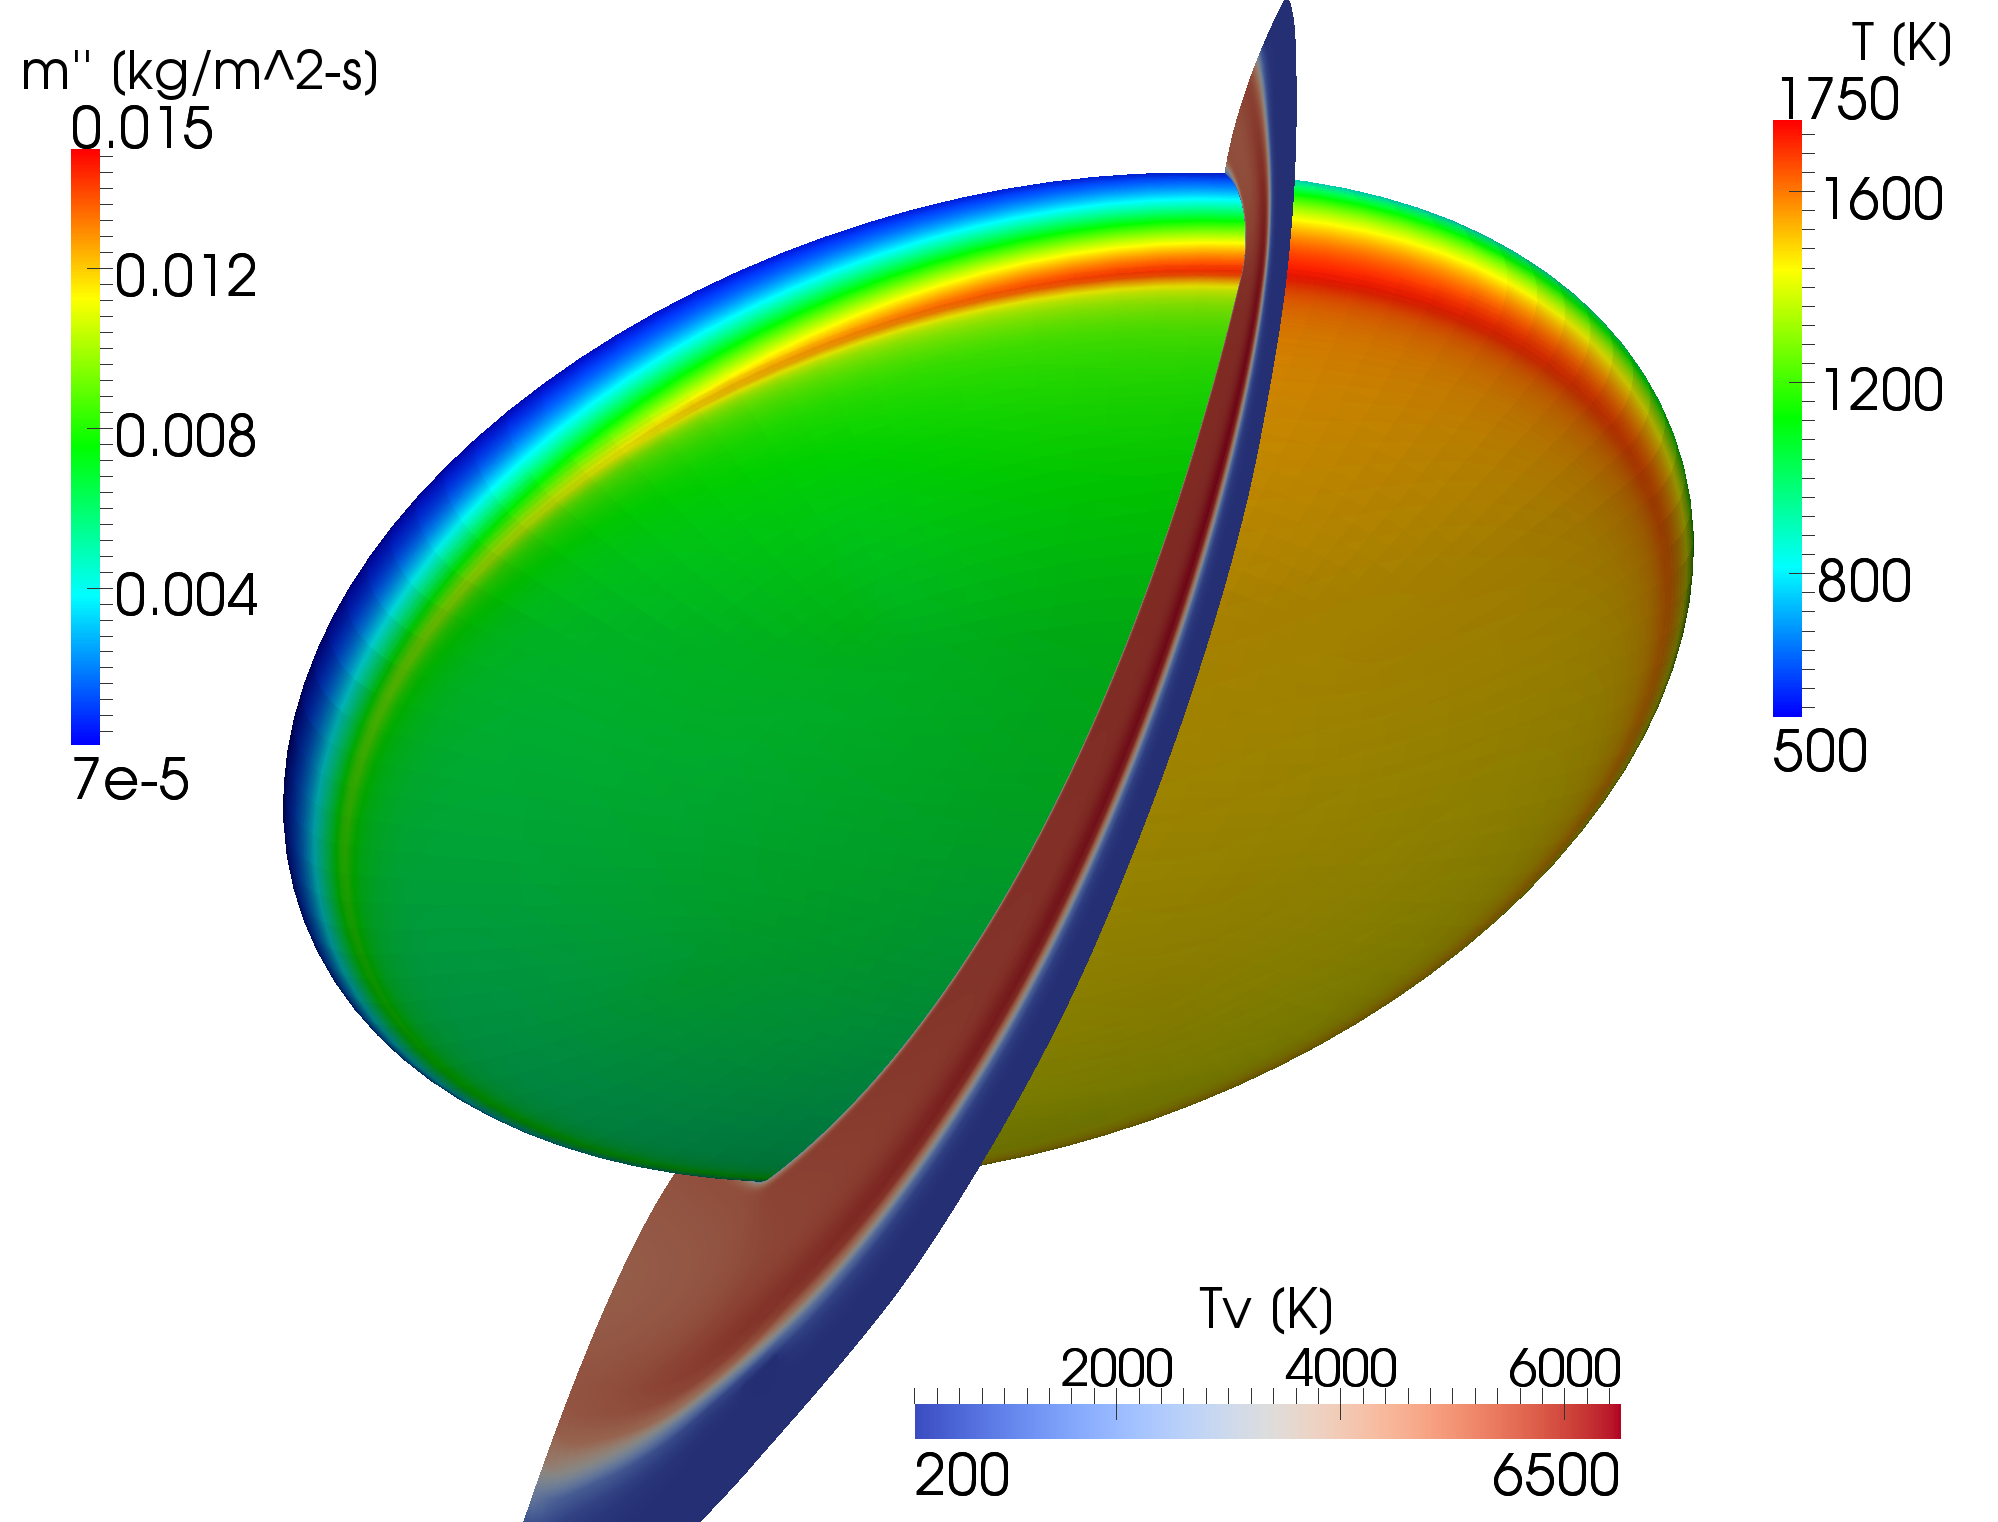
\includegraphics[width=.45\textwidth]{ablating_hs_wbg}
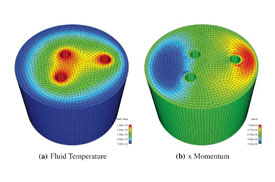
\includegraphics[width=.55\textwidth]{moose}
\end{columns}

\begin{columns}
\column{.35\textwidth}
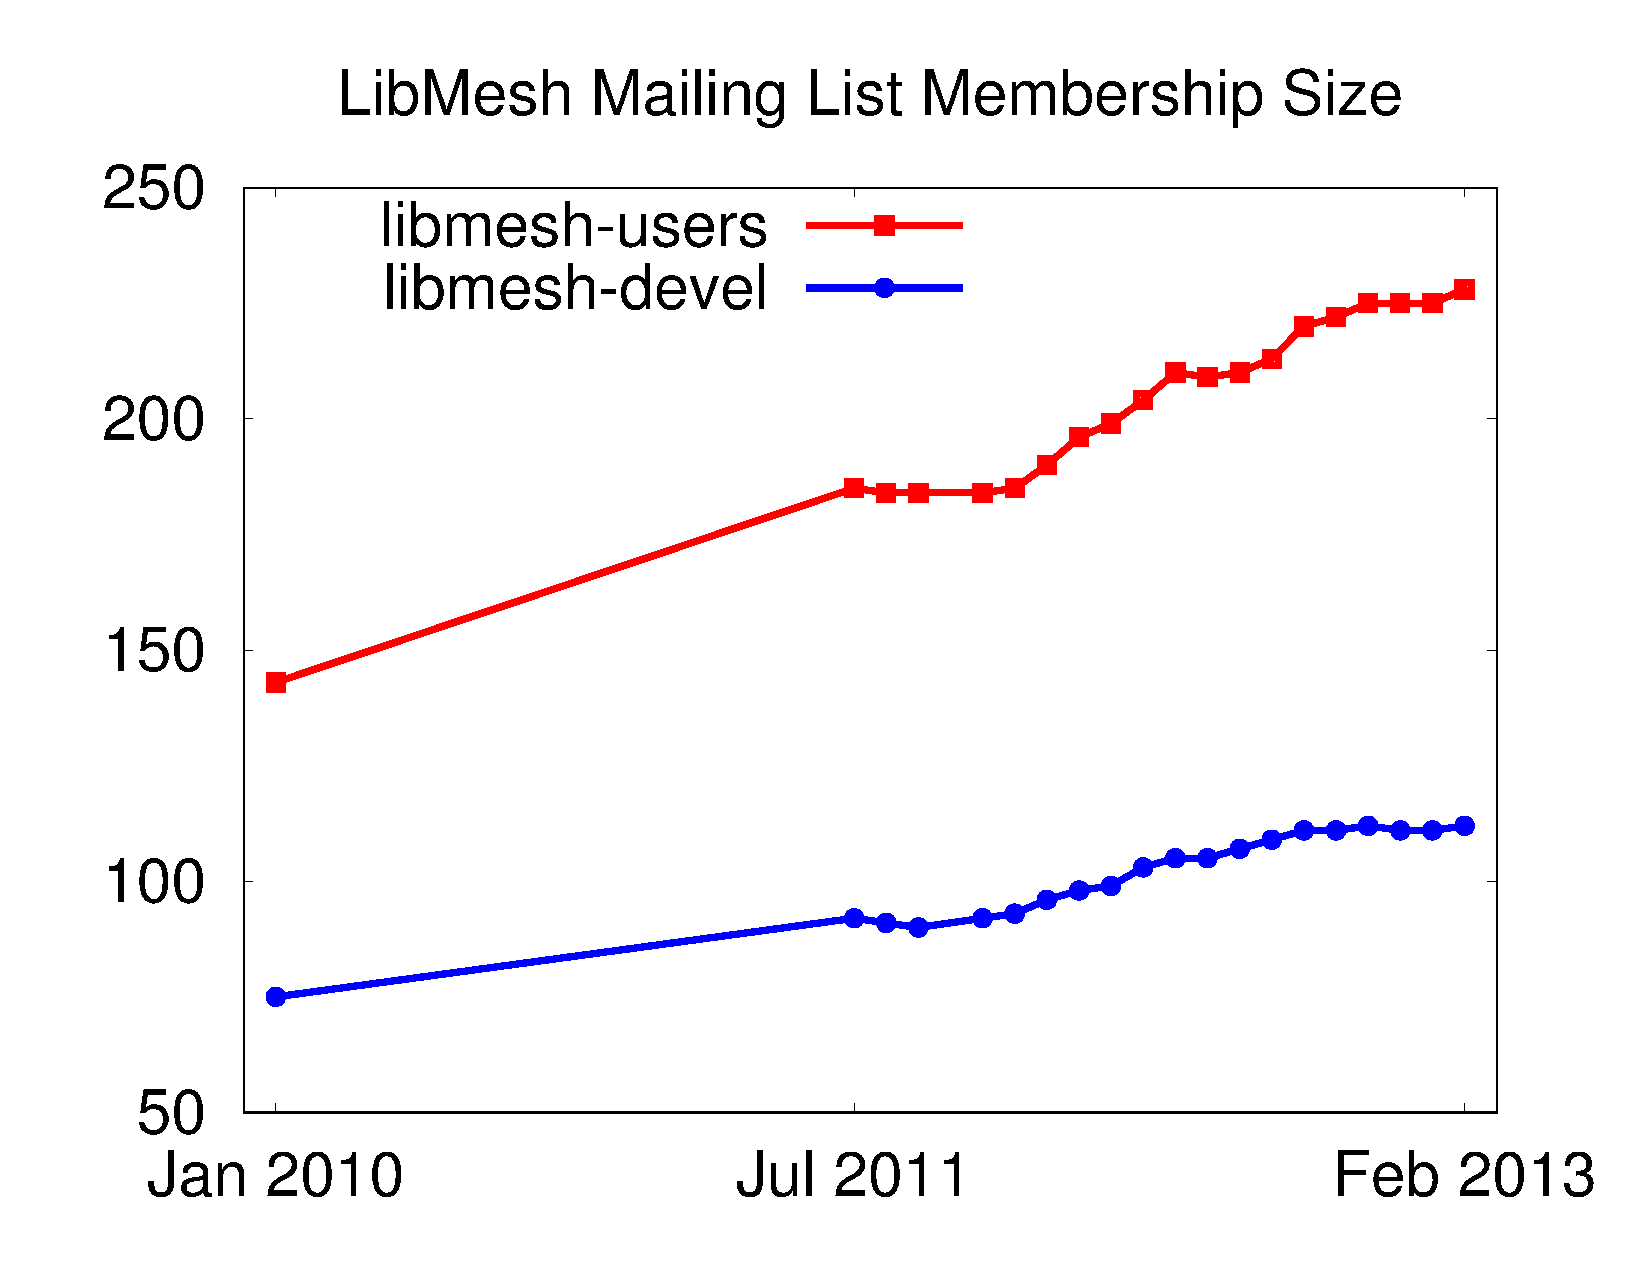
\includegraphics[width=\textwidth]{libmesh_mailinglists_membership}

\column{.65\textwidth}
\begin{block}{Challenges}
\begin{itemize}
\item Widely dispersed core developers
\begin{itemize}
\item INL, UT-Austin, JSC, MIT, Harvard, Argonne
\end{itemize}
\item ITAR, Commercial applications common
\item Radically different application types
\end{itemize}
\end{block}
\end{columns}

\end{frame}


\section{Collaboration Strategies}
% email
% github issues
% ticketing systems on Trac/buildbot
% Pushing patches into repo forks, pull requests
% Sharing patches?


%===============================================================================
% NEW SLIDE
%===============================================================================
\begin{frame}
\frametitle{Collaboration Strategies}

\begin{block}{Communication}
\begin{itemize}
	\item Face to face, instant messaging, teleconference
	\item Email lists
	\begin{itemize}
		\item \texttt{libmesh-users@sourceforge.net},
			\texttt{libmesh-devel@sourceforge.net}
	\end{itemize}
	\item Trac tickets, Redmine issues
	\item SourceForge, GitHub issues
\end{itemize}
\end{block}

\begin{block}{Code}
\begin{itemize}
	\item Email attachments
	\item Ticket attachments
	\begin{itemize}
		\item Repository forks!
		\item Pull requests!
	\end{itemize}
\end{itemize}
\end{block}

\end{frame}



\section{API Development}

\begin{frame}[fragile]
\frametitle{Tracking API Changes}

\begin{block}{API versions easily proliferate...}
%\begin{minted}[fontsize=\footnotesize]{c++}
\small
\begin{semiverbatim}
#if PETSC_VERSION_LESS_THAN(3,1,0)
  ierr = MatGetSubMatrix(matrix->mat(),
           _restrict_to_is, _restrict_to_is_complement,
           \alert{PETSC_DECIDE}, MAT_INITIAL_MATRIX, &submat1);
#else
  ierr = MatGetSubMatrix(matrix->mat(),
           _restrict_to_is, _restrict_to_is_complement,
           MAT_INITIAL_MATRIX, &submat1);
#endif
\end{semiverbatim}
%\end{minted}
\end{block}

\begin{itemize}
	\item Maintain a wide range of external compatibility
	\item Limit \libmesh{} API changes
\end{itemize}

\end{frame}

\begin{frame}
\frametitle{Signaling API Changes}
\begin{block}{Development practices}
\begin{itemize}
	\item Old, new APIs {\emph{overlap}}
	\item Easier with C++ function overloading, default arguments
	\begin{itemize}
		\item Adding \texttt{f(a,b)} does not preclude keeping
			\texttt{f(a)}
		\item Adding \texttt{f(a,b=default)} can replace
			\texttt{f(a)}
	\end{itemize}
\end{itemize}
\end{block}

\begin{block}{Runtime warnings}
\begin{itemize}
	\item {\texttt{libmesh\_experimental()}} \quad (in-flux APIs)
	\item {\texttt{libmesh\_deprecated()}} \quad (~1 year, 1-2 releases)
\end{itemize}
\end{block}

\begin{block}{Examples}
\begin{itemize}
	\item {\texttt{OStringStream} workaround class}
	\item {\texttt{Parallel::} global functions}
\end{itemize}
\end{block}


\end{frame}


\section{Source Code Control}

\begin{frame}{}
  \begin{itemize}\itemsep=.05\textheight
  \item When discussing SCC software, the distinction between ``distributed'' and ``centralized''
    is often stressed, perhaps unnecessarily. 
  \item Distributed SCC software, like \texttt{git}, is very frequently used in a semi-centralized manner.
  \item The \libmesh library is now distributed from GitHub\footnote{\url{https://github.com/libMesh/libmesh}},
    and therefore we focus on \texttt{git} in this talk, but the discussion should apply to other
    SCC software as well.
  \end{itemize}
\end{frame}


\subsection{Attention Deficit Development}
\begin{frame}
  \begin{itemize}\itemsep=.05\textheight
  \item A more intrinsic difference between various flavors of SCC software is rather the ability to
    make ``local commits.''
  \item \texttt{git} and other ``distributed'' SCC software packages (\texttt{hg}) have this feature.
  \item SVN lacks this feature, and therefore makes work interruptions (which can be rather frequent in 
    collaborative development) difficult to handle.
  \end{itemize}
\end{frame}



\begin{frame}
  \begin{itemize}\itemsep=.05\textheight
  \item Consider the following scenario: 
    \begin{itemize}
    \item You are working on a new feature and have several locally-modified
      files (``A'', ``D'', or ``M'' state in \texttt{svn status})
    \item You receive email from a collaborator about a bug fix he'd like you to test ASAP.
      His patch may or may not conflict with your current set of changes.
    \end{itemize}
  \item What do you do?
  \end{itemize}
\end{frame}


\begin{frame}
  \begin{itemize}\itemsep=.05\textheight
  \item In SCC software without local commits, your choices are:
      \begin{enumerate}
      \item Make a patch of your local changes (e.g.\ \texttt{svn diff}), revert them, and hope to come back to them later.
      \item See if your collaborator's patch applies cleanly on top of what you are already doing.
      \item Create a fresh checkout, apply the patch, recompile everything, and test.
      \end{enumerate}
  \item The choices aren't pretty:
    \begin{enumerate}
    \item This is manual source code control, something tools should help you avoid!
    \item If the patch program fails, the results can be cryptic; if patch succeeds, it may be hard to revert later.
    \item This approach clearly doesn't scale in disk space or CPU cycles.
    \end{enumerate}
  \end{itemize}
\end{frame}


\begin{frame}
  \begin{itemize}\itemsep=.05\textheight
  \item In SCC software with local commits, specifically \texttt{git}, 
    and assuming you are working on \texttt{my-branch}, you:
      \begin{itemize}
      \item \texttt{git ci} your work.
      \item Create a new branch, probably from \texttt{master}.
      \item Apply your collaborator's patch, let him know what you find.
      \item \texttt{git co my-branch}
      \end{itemize}

    \item Once you are back on \texttt{my-branch}, you can do a ``soft reset'' to get back to exactly
      where you were before the interruption.

%    \item You can delete your collaborator's branch, or leave it lying around in case he sends you another patch.

    \item If you don't want to mess with extra branches, you can instead \texttt{git stash} what you're currently
      doing, try out your collaborator's patch, and \texttt{git stash pop} to return to your original state.
  \end{itemize}
\end{frame}




\subsection{Linear and Nonlinear History}

\begin{frame}{}
  \begin{itemize}\itemsep=.05\textheight
  \item The first question a \texttt{git}-based development team\footnote{Especially teams transitioning from SVN.} should debate
    is whether maintaining a ``linear'' history is desirable/important.
  \item There are pros and cons to both linear and nonlinear development histories.
  \item The answer probably lies somewhere between ``rigidly-enforced linearity'' and ``merges gone wild.''
  \end{itemize}
\end{frame}


\begin{frame}[fragile]{Example - Useful Nonlinearity}
\small
\begin{semiverbatim}
* 4df7f73 Adding list of bibtex templates.
*   e04db6d Merge pull request #45 from benkirk/eigen
|\\  
| * e3bd55d get contributed Eigen into build system
| * 13fa33d add eigen-3.1.2 unsupported API
| * d03f946 adding eigen-3.1.2 to contrib
|/  
* 1249c5d more fine-grained fallback for --disable-mpi
* e15fef7 use <rpc/xdr.h> when it is there
\end{semiverbatim}
\begin{itemize}
\item A (short-lived) feature branch is created, committed to, and merged back into master.
\item Preserves the context in which development took place.  Useful!
\end{itemize}
\end{frame}



\begin{frame}[fragile]{Example - Rigid Linearity}
\small
\begin{semiverbatim}
* bc56be9 Fixes for our Epetra vector interface
* 4f2b016 Making reading work, adding support \ldots
* 243753e Again, don't degrade to single precision \ldots
* b277d0a We are using a vtkDoubleArray, so don't \ldots
* 6bac31a Hoist function calls out of loop conditionals.
* fe85fae Standardizing spacing, formatting, indentation, etc.
* ce703f9 Use VTK_LEGACY_REMOVE.  Thanks, cato-, for the idea.
* 84da4b4 prevent netcdf from running most of the \ldots
\end{semiverbatim}
\begin{itemize}
\item Commits \texttt{fe85fae} --- \texttt{4f2b016} are a group of logically-connected changes.
\item This information is lost because the author did his development directly on master instead of branching.
\end{itemize}
\end{frame}





\begin{frame}[fragile]{Example - Misleading Nonlinearity}
\small
\begin{semiverbatim}
*   cfd23fa Merge branch master
|\\  
| * 285ebaa Adding citations and webpage generation script.
* | 1aa5d5f trump --enable-petsc with --disable-mpi
* | 9644c5f fallback to rpc/xdr.h when looking for xdr.
|/  
* 070515a LibMeshInit can accept more argument constness
\end{semiverbatim}
\begin{itemize}
\item The three ``middle'' commits are unrelated to one another.
\item The author of \texttt{9644c5f} and \texttt{1aa5d5f} ran \texttt{git pull}, bringing
  down an unrelated change, and producing a merge commit.
\item Branch does not preserve any particular development context.
\end{itemize}
\end{frame}


\begin{frame}[fragile]{Example - Merges Gone Wild}
\small
\begin{semiverbatim}
*   9f639a6 Merge branch master
|\\  
| *   936e197 Merge branch master
| |\\  
| | * 2b80c18 Remove uninitialized dphi warnings \ldots
| * | 0309eac is_adjoint() bugfixes
| |/  
* | 514052e UnsteadySolver fixes and optimization
* |   e5aac7b Merge branch master
|\\ \\  
| |/  
| * b6155a5 Changes in quadrature_simpson_3D.C for -Wshadow.
\end{semiverbatim}
  \begin{itemize}
  \item Three ``merge'' commits and four ``real'' commits.
  \item High signal-to-noise ratio.
  \item \texttt{git bisect} often stops at merge commits.
  \end{itemize}
\end{frame}


\begin{frame}{Current Guidelines}
  \begin{itemize}\itemsep=.05\textheight
  \item Strive for ``useful nonlinearity.''
  \item Develop separate feature sets on separate branches; merge them back to master when complete.
  \item Minimize or eliminate periodic/unnecessary merge commits.
  \item Instead, \texttt{rebase} feature branches on top of master before merging and pushing
  \item Rebasing public (aka shared) branches is bad\texttrademark, so wait until you are ready to push,
    branch from the shared branch locally, rebase it on top of master, and then merge it.
  \end{itemize}
\end{frame}



%\subsection{Is Git Complicated?}
\begin{frame}[fragile]
  \begin{columns}
    \column{.48\textwidth}
    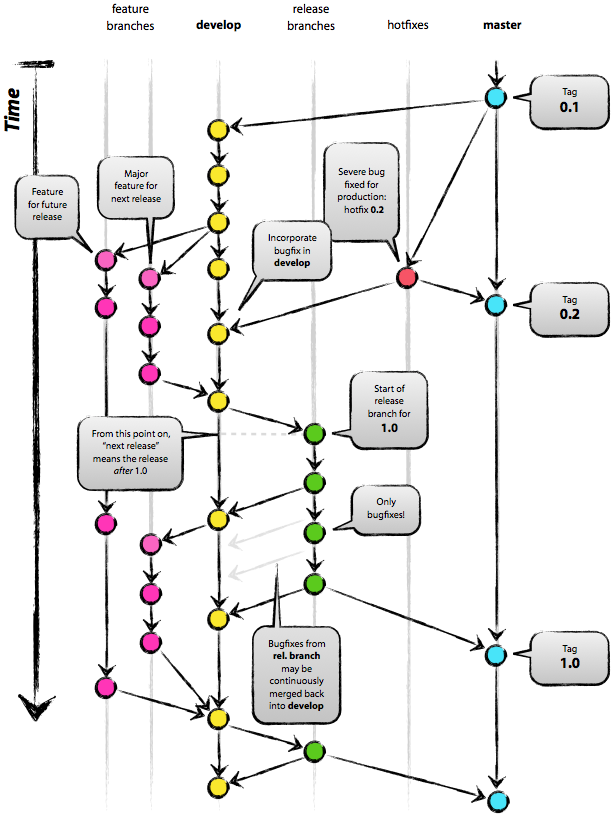
\includegraphics[width=\textwidth]{git_branching}
    \column{.48\textwidth}
    \begin{itemize}\itemsep=.05\textheight
    \item \texttt{git} can be complicated, but it is not inherently so.
    \item Forget cats, there is more than one way to skin every type of animal in \texttt{git}.
    \item Teams should find the approach that works best for them.
    \end{itemize}
  \end{columns}
    \small
    \begin{itemize}
    \item \url{http://nvie.com/posts/a-successful-git-branching-model}
    \end{itemize}
\end{frame}


\section{Development and Testing}

\begin{frame}
  \frametitle{Software Tracking}
  \begin{itemize}\itemsep=.05\textheight
  \item Trac, Redmine - Wiki and issue tracking systems for software development projects
    \begin{itemize}
    \item \url{http://trac.edgewall.org}, \url{http://www.redmine.org}
    \item Interface to your VCS of choice
    \item Issue tracking (aka tickets) can reference commits and vice versa
    \item Open source: (BSD, GPL2)
    \end{itemize}
  \item Bitten, BuildBot - Continuous Integration
    \begin{itemize}
    \item \url{http://bitten.edgewall.org}, \url{http://trac.buildbot.net}
    \item Build recipes in XML, Python formats
    \item Can send build failure notifications directly to relevant parties
    \end{itemize}
  \end{itemize}
\end{frame}



% This is a MOOSE-specific ticket, find a libmesh one. 
% \begin{frame}{Issue tracking (tickets)}
%   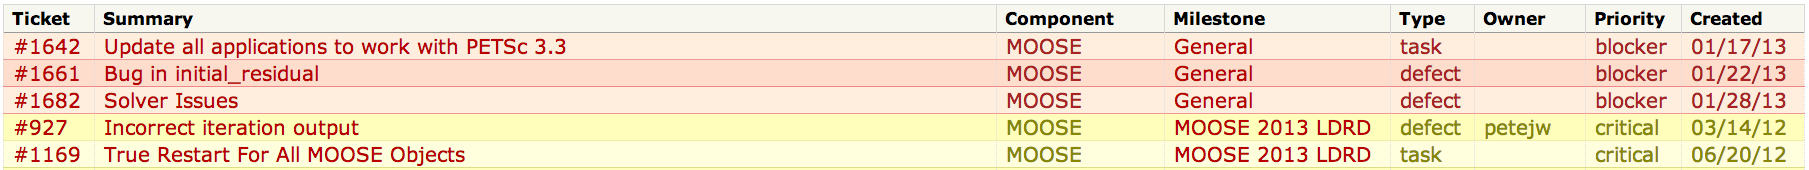
\includegraphics[width=\textwidth]{moose_tickets}
%   \\
%   \vspace{.01\textheight}
%   \begin{center}
%     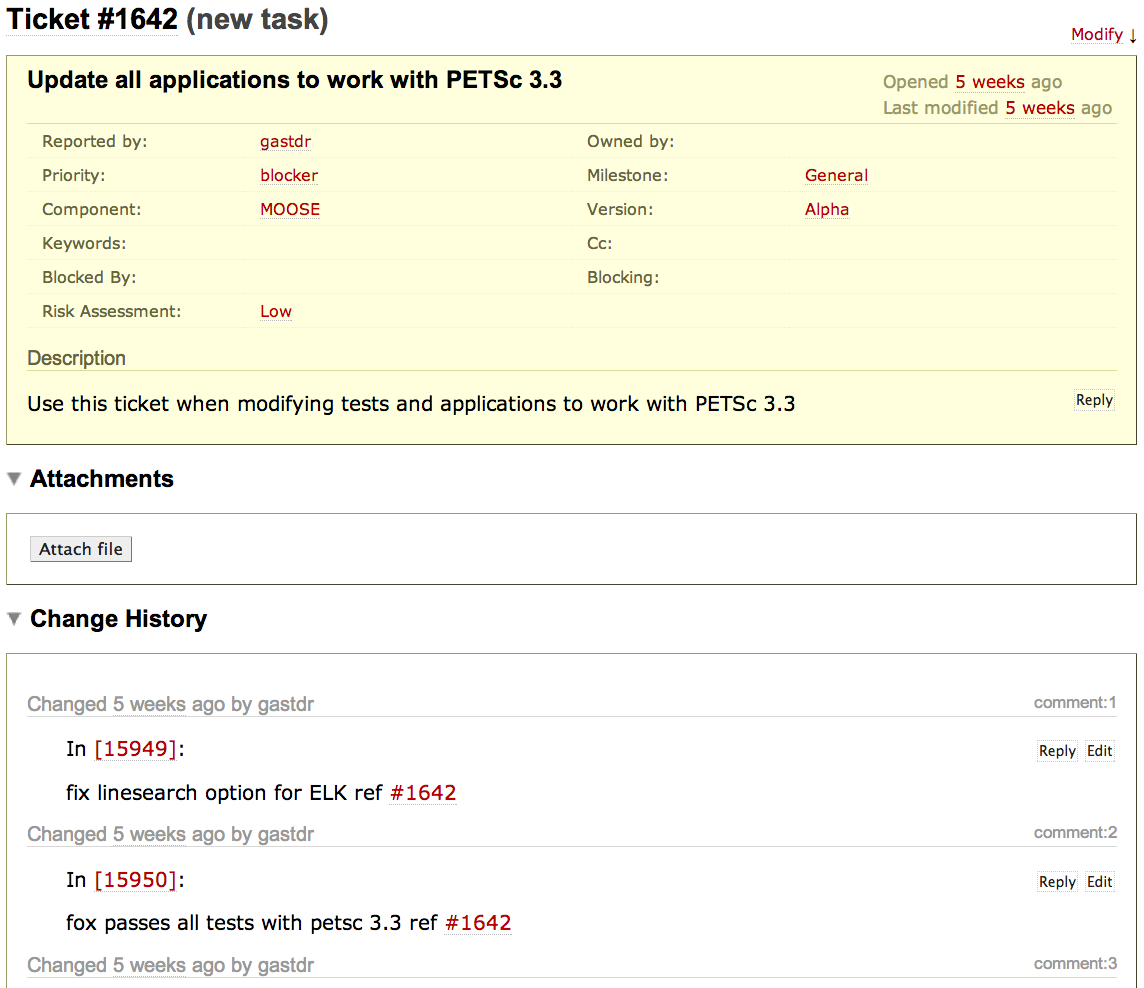
\includegraphics[width=.55\textwidth]{ticket_1642}
%   \end{center}
% \end{frame}


% This ticket does not show integration with SCC.
% \begin{frame}{Issue tracking (tickets)}
%   \begin{center}
%     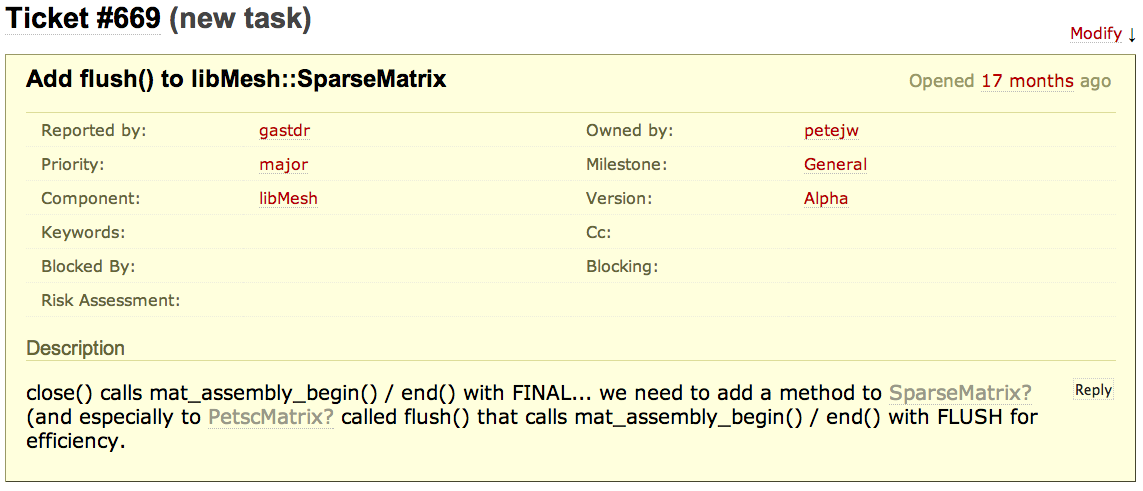
\includegraphics[width=.95\textwidth]{ticket_669}
%   \end{center}
% \end{frame}

% Again, not really a libmesh ticket, but something that broke in MOOSE
% because of changes to periodic BCs in libmesh...
\begin{frame}{Issue tracking (tickets)}
  % Slide notes:
  % * Tickets can have a reporter, owner, category, priority, and milestone they are tied to.
  % * All interested parties can be notified whenever the status of a ticket changes.
  \begin{center}
    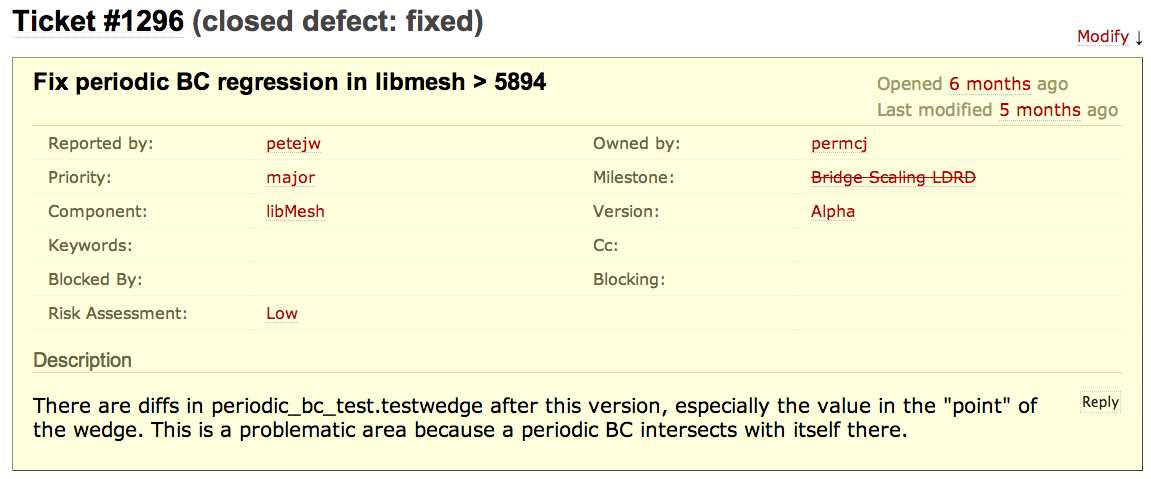
\includegraphics[width=.95\textwidth]{ticket_1296_top}
  \end{center}
\end{frame}

\begin{frame}{Issue tracking (tickets)}
  % Slide notes:
  % * You can reference tickets from commit messages, and they will automatically show up as 
  %   comments on the ticket.
  % * Putting e.g. "closes #1296" in your commit message automatically closes the ticket on Trac.
  % * The commit revision also gets linked in the ticket comment, so you can click and see the diff.
  % * Links for closed tickets show up with a strikethrough.
  % * Later commits, e.g. 12713, can still reference tickets that have been closed.
  \begin{center}
    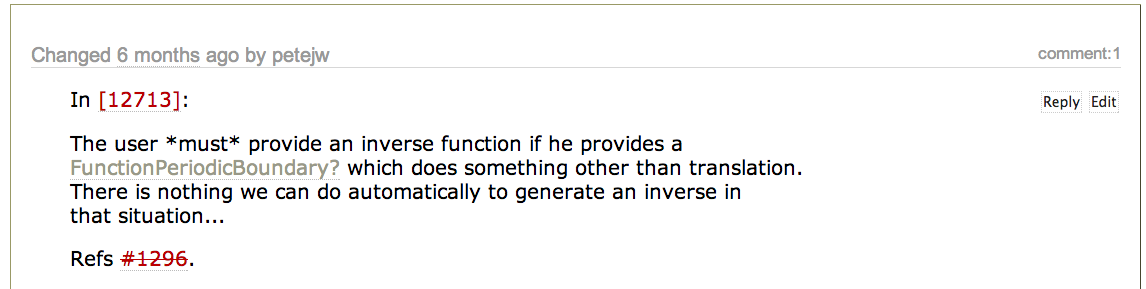
\includegraphics[width=.95\textwidth]{ticket_1296_bot1}
    \\
    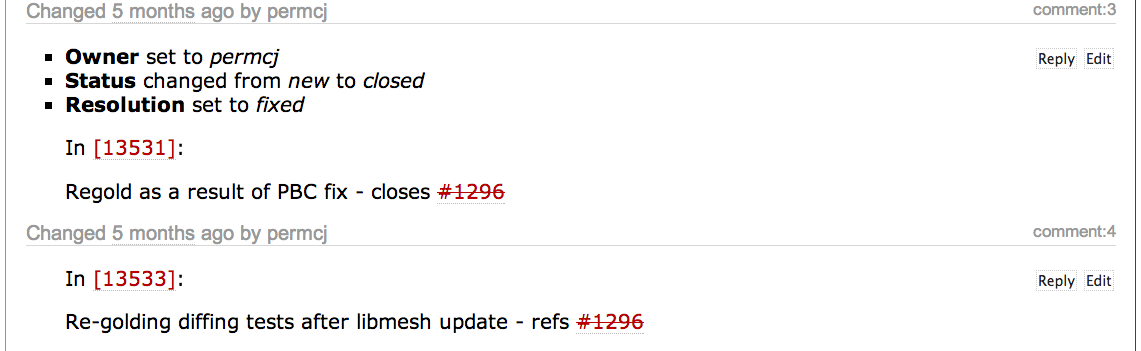
\includegraphics[width=.95\textwidth]{ticket_1296_bot2}
  \end{center}
\end{frame}





\begin{frame}{Build Status}
  % Slide notes:
  % * The build status for commit 16927 on some architectures is shown
  % * Green box means the build succeeded on that architecture
  % * When the build succeeds, Trac automatically merges the revision into "MOOSE-stable"
  % * In this case, commit 16927 gets merged into stable as version 16931 (stable 
  %   and dev are in the same repo other commits may occur during the build)
  % * Note also, the commit message closes a ticket that is also stored in the Trac system
  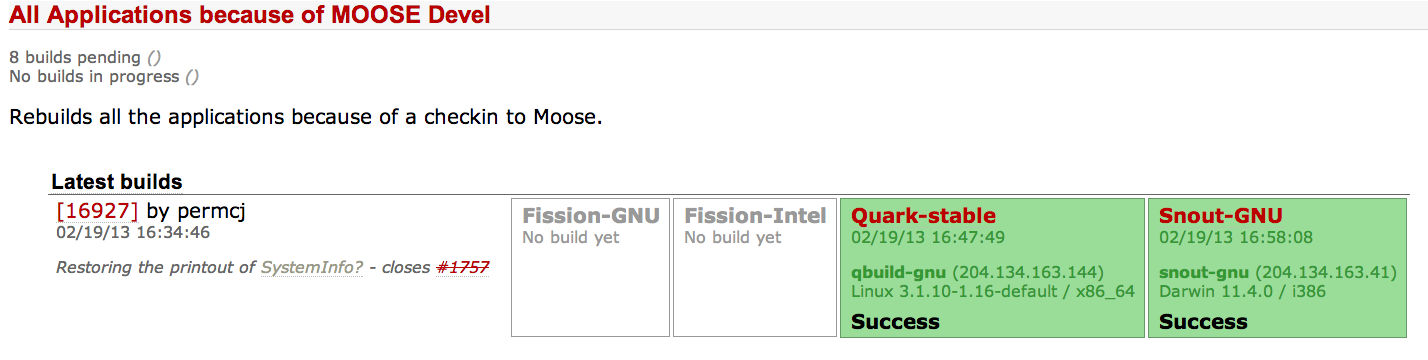
\includegraphics[width=\textwidth]{buildstatus_top}
  \\
  \vspace{.01\textheight}
  \begin{center}
    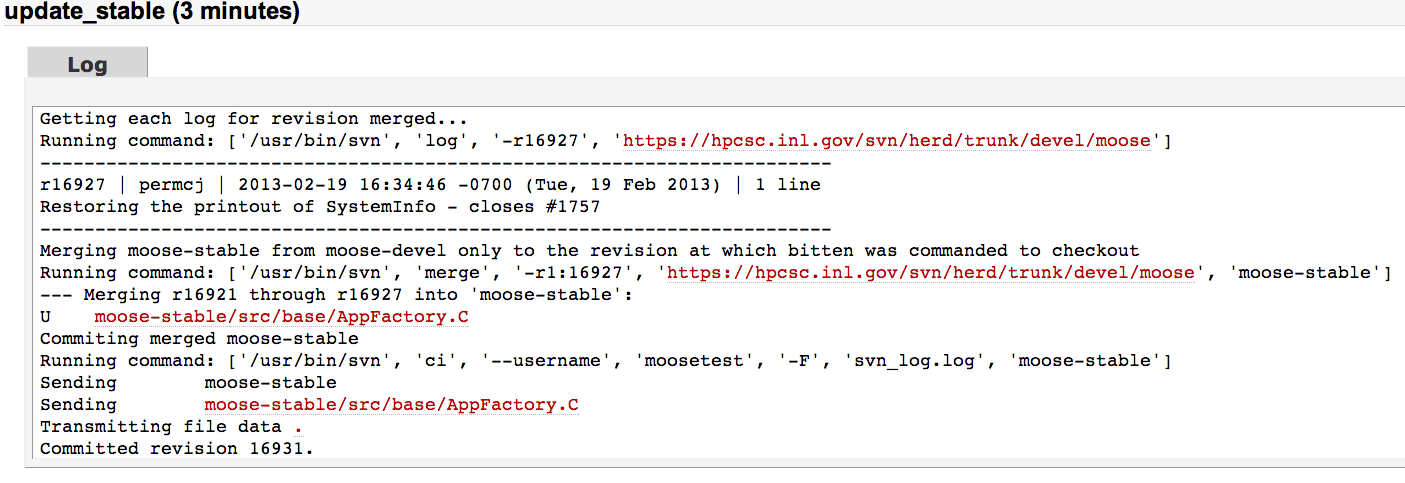
\includegraphics[width=\textwidth]{updatestable_log}
  \end{center}
\end{frame}



\begin{frame}[t]{Regression Testing}
  % Slide notes:
  % * MOOSE (and dependent apps) have regression test suites which must all pass before a commit
  %   is allowed to merge into MOOSE-stable
  % * Shown on the right is a summary of the regression tests for MOOSE itself.
  % * The tests are all designed to be relatively "fast" (and can be run in parallel) so the CI system doesn't get bogged down.
  \begin{columns}
    \column{.2\textwidth}
    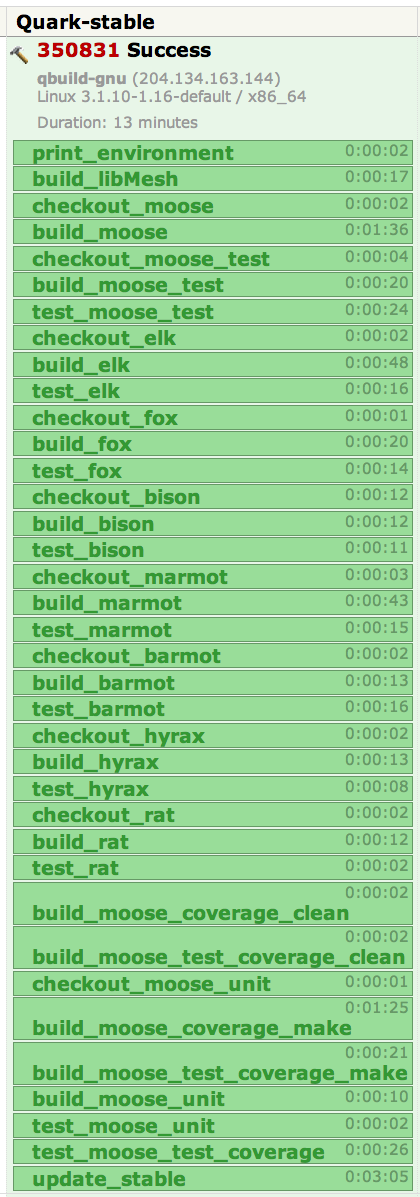
\includegraphics[width=\textwidth]{quark_stable_summary}

    \column{.75\textwidth}
    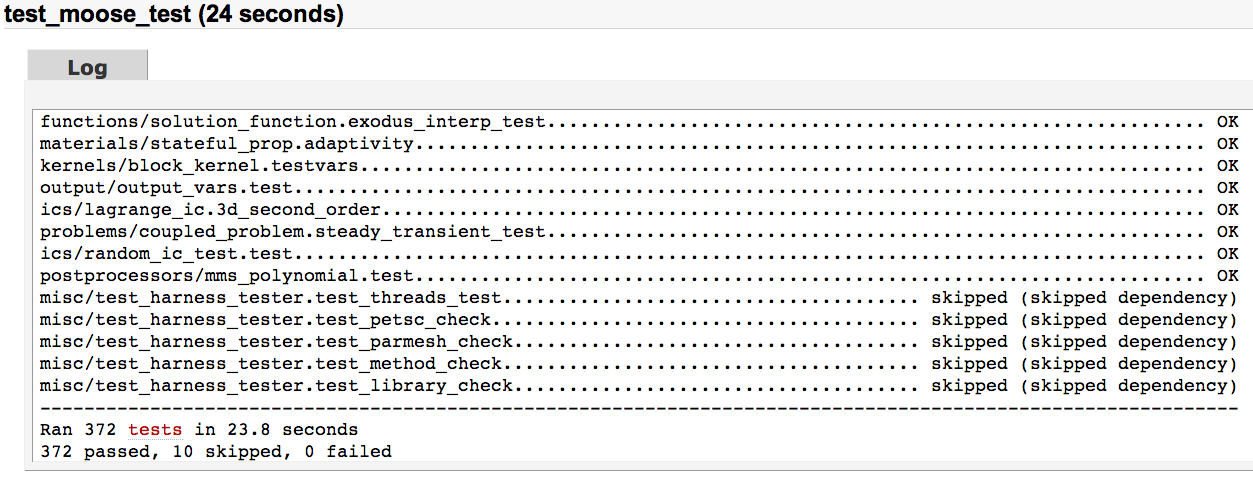
\includegraphics[width=\textwidth]{moosetest_log}
  \end{columns}
\end{frame}


\begin{frame}{Diagnosing Failed Builds}
  % Slide notes:
  % * When a build fails, Trac can also help you diagnose the problem.
  % * In this particular case, the error was a wrong include path.
  % * After fixing it up and recommitting, the continuous integration cycle begins again...
  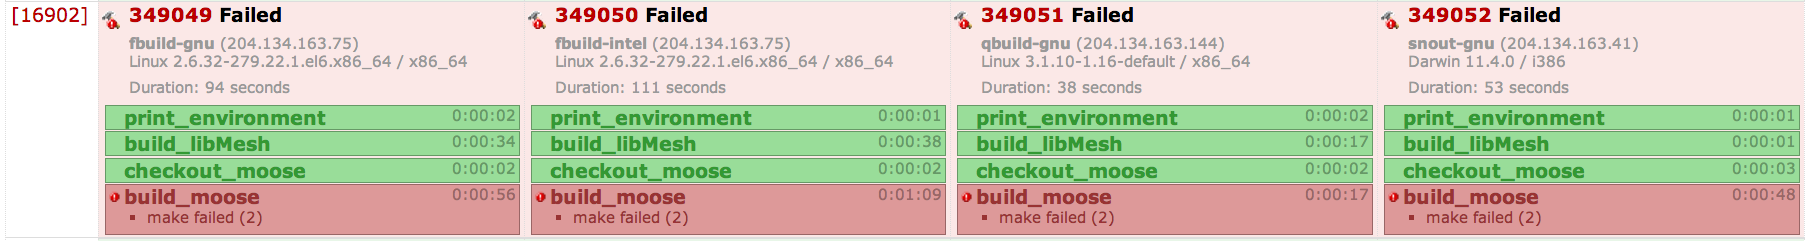
\includegraphics[width=\textwidth]{failed_build}
  \\
  \vspace{.1\textheight}
  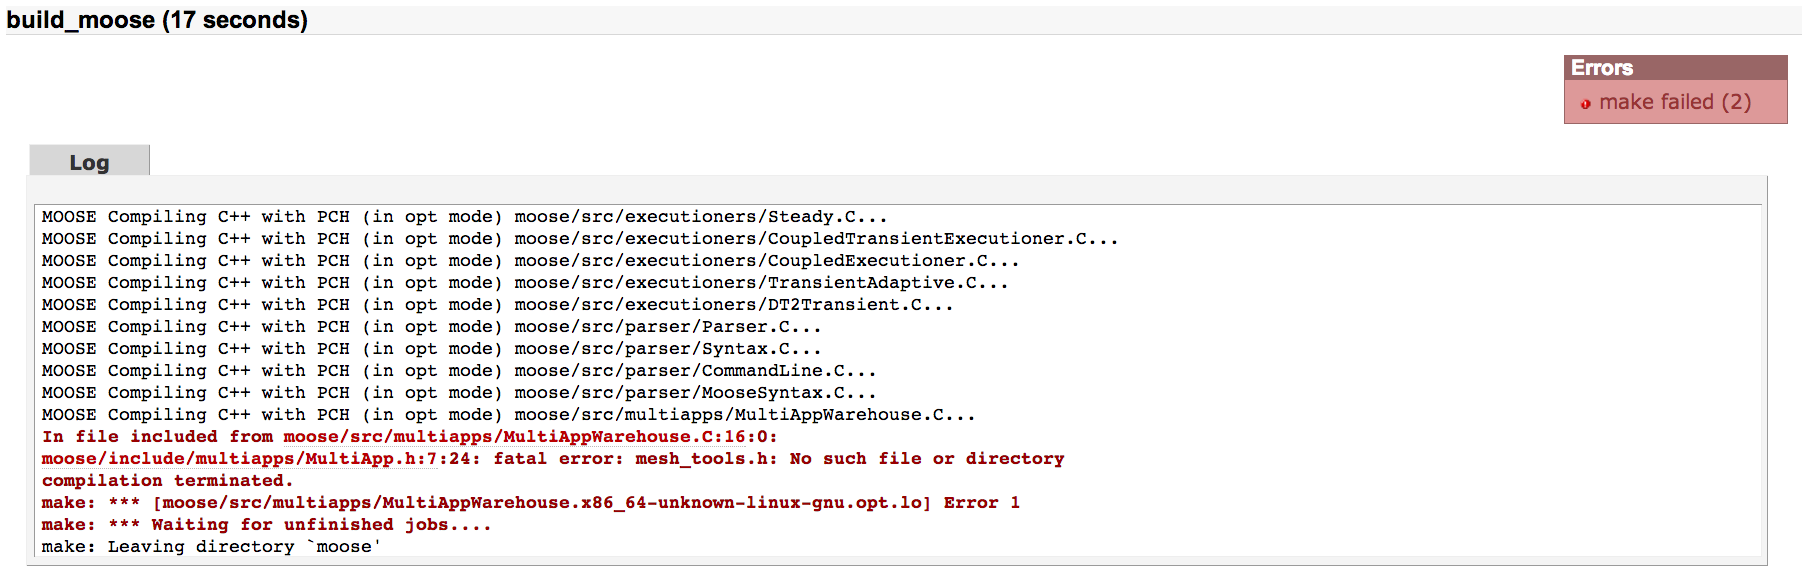
\includegraphics[width=\textwidth]{failed_build_details}
\end{frame}


% Buildbot?

\section{Build Systems}

\begin{frame}{Autotools, Pros and Cons}
  % Slide notes:
  % * We've been using autoconf forever
  % * Automake, libtool are much more recent, more controversial
  % * We looked at scons, cmake
  % * We keep bootstrap output in git so RCS users don't need automake
  % * But now build system changes are much more annoying
\begin{columns}
\column{.5\textwidth}
\begin{block}{Autoconf}
	\begin{itemize}
		\item \pro{Manages feature selection}
			\begin{itemize}
				\item 50+ {\texttt{--enable-foo}} options
			\end{itemize}
		\item \pro{Portability tests, workarounds}
		\item \con{POSIX shell dependence}
	\end{itemize}
\end{block}

\begin{block}{Libtool}
	\begin{itemize}
		\item \pro{Easily used via automake}
		\item \pro{Broader shared library support}
		\item \pro{DLL management in install}
		\item \con{More difficult in-place debugging}
	\end{itemize}
\end{block}

\column{.4\textwidth}
\begin{block}{Automake}
	\begin{itemize}
		\item \pro{dist, check, install targets}
		\item \pro{Out-of-source builds}
		\item \pro{\emph{Standardized conventions}}
		\item \con{More difficult METHOD support}
		\item \con{``bootstrap'' process}
		\begin{itemize}
			\item \con{Do users have autotools?}
			\item \con{Custom scripts for libMesh}
		\end{itemize}
	\end{itemize}
\end{block}

\end{columns}

\end{frame}

%===============================================================================
% NEW SLIDE
%===============================================================================
\begin{frame}
\frametitle{}
\begin{columns}[c] 
\begin{column}{.5\textwidth} 
\begin{block}{}
\center{Questions?}
\end{block}
\end{column}
\end{columns}
\begin{center}
\end{center}
\end{frame}

 
\end{document}

% LocalWords:  SVN df bibtex benkirk eigen bd API contrib mpi fef rpc
% LocalWords:  cfd ebaa webpage aa petsc xdr LibMeshInit constness bc
% LocalWords:  dphi eac adjoint bugfixes UnsteadySolver aac simpson
% LocalWords:  Wshadow Nonlinearity Epetra vtkDoubleArray bac fe fae
% LocalWords:  ce VTK cato da netcdf SCC GitHub nonlinearity rebase
% LocalWords:  Rebasing hg svn ci Trac versa
